\documentclass[twoside,11pt]{article}

\usepackage{graphicx}
\pagestyle{myheadings}

% +
%  Name:
%     sc19.tex
%
%  Purpose:
%     The SMURF SCUBA-2 data analysis cookbook (SC/19)
%
%  Authors:
%     Ed Chapin (UBC)
%
%  Copyright:
%     Copyright (C) 2009 University of British Columbia
%
%  History:
%     2009-05-22 (EC):
%        Original version, borrowing from SC11
%     2009-06-04 (EC):
%        Changed to SC19 from SC18 to avoid conflict with X-ray cookbook
%     {Add further history here}
%
% -

% ------------------------------------------------------------------------


% Add any \newcommand or \newenvironment commands here
\newcommand{\about}{$\sim$}
\newcommand{\eg}{{\it e.g.}}
\newcommand{\ie}{{\it i.e.}}
\newcommand{\micron}{\mbox{\,${\mu}$m}}            % microns
\newcommand{\arcmin}{{$^\prime$}}
\newcommand{\degr}{\mbox{\,$^\circ$}}               % degrees sign
% ------------------------------------------------------------------------



% ------------------------------------------------------------------------


% ? Document identification
\newcommand{\stardoccategory}  {Starlink Cookbook}
\newcommand{\stardocinitials}  {SC}
\newcommand{\stardocsource}    {sc\stardocnumber}
\newcommand{\stardocnumber}    {19.01}
\newcommand{\stardocauthors}   {E. Chapin \\ 
University of British Columbia}
\newcommand{\stardocdate}      {22 May 2009}
\newcommand{\stardoctitle}     {The SMURF SCUBA-2 data analysis cookbook}
\newcommand{\stardocversion}   {\ }
\newcommand{\stardocmanual}    {\ }
\newcommand{\stardocabstract}  {[Text of abstract]}
% ? End of document identification
 
% A new environment for quoting verbatim
% Environment for indenting and using a small font.
\newenvironment{myquote}{\begin{quote}\begin{small}}{\end{small}\end{quote}}
 


\newcommand{\text}[1]{{\small \texttt{#1}}}
 
% SCUBA reference
%\newcommand{\scuba}{\htmladdnormallink{SCUBA}{http://www.jach.hawaii.edu/JCMT/}}

 
% Starlink Package names
\newcommand{\starlink}{\htmladdnormallink{Starlink}{http://star-www.rl.ac.uk/}} 

% set up some common package names
\newcommand{\Kappa}{\xref{\textsc{Kappa}}{sun95}{}}
\newcommand{\Figaro}{\xref{\textsc{Figaro}}{sun86}{}}
\newcommand{\gaia}{\xref{\textsc{Gaia}}{sun214}{}}
\newcommand{\convert}{\xref{\textsc{Convert}}{sun55}{}}
\newcommand{\fluxes}{\xref{\textsc{Fluxes}}{sun213}{}}
\newcommand{\ccdpack}{\xref{\textsc{Ccdpack}}{sun139}{}}
\newcommand{\Iras}{\xref{\textsc{Iras90}}{sun163}{}}
\newcommand{\ndf}{\xref{NDF}{sun33}{}}
\newcommand{\agi}{\xref{AGI}{sun48}{}}
\newcommand{\surf}{\xref{\textsc{Surf}}{sun216}{}}
\newcommand{\Specdre}{\xref{\textsc{Specdre}}{sun140}{}}
\newcommand{\jcmtdr}{\xref{\textsc{JCMTdr}}{sun132}{}}
\newcommand{\nod}{\textsc{nod2}}
\newcommand{\ESP}{\xref{ESP}{sun180}{}}
\newcommand{\GKS}{\xref{GKS}{sun83}{}}
\newcommand{\oracdr}{\xref{\textsc{orac-dr}}{sun231}{}}
\newcommand{\smurf}{\xref{\textsc{Smurf}}{sun258}{}}

% Application tasks
\newcommand{\task}[1]{\textsf{#1}}
 
% ADAM parameters
\newcommand{\param}[1]{\texttt{#1}}
 
% SMURF tasks
\newcommand{\concat}{\xref{\task{sc2concat}}{sun258}{SC2CONCAT}}
\newcommand{\fft}{\xref{\task{sc2fft}}{sun258}{SC2FFT}}
\newcommand{\clean}{\xref{\task{sc2clean}}{sun258}{SC2CLEAN}}
\newcommand{\flatfield}{\xref{\task{flatfield}}{sun258}{FLATFIELD}}
\newcommand{\makemap}{\xref{\task{makemap}}{sun258}{MAKEMAP}}
\newcommand{\jcmtstate}{\xref{\task{jcmtstate2cat}}{sun258}{JCMTSTATE2CAT}}
 
% Non surf tasks

% KAPPA 
\newcommand{\qualtobad}{\xref{\task{qualtobad}}{sun95}{QUALTOBAD}}
\newcommand{\showqual}{\xref{\task{showqual}}{sun95}{SHOWQUAL}}
\newcommand{\display}{\xref{\task{display}}{sun95}{DISPLAY}}
\newcommand{\aperadd}{\xref{\task{aperadd}}{sun95}{APERADD}}
\newcommand{\linplot}{\xref{\task{linplot}}{sun95}{LINPLOT}}
\newcommand{\mlinplot}{\xref{\task{mlinplot}}{sun95}{MLINPLOT}}
\newcommand{\drawsig}{\xref{\task{drawsig}}{sun95}{DRAWSIG}}
\newcommand{\centroid}{\xref{\task{centroid}}{sun95}{CENTROID}}
\newcommand{\hislist}{\xref{\task{hislist}}{sun95}{HISLIST}}
\newcommand{\globals}{\xref{\task{globals}}{sun95}{GLOBALS}}
\newcommand{\setaxis}{\xref{\task{setaxis}}{sun95}{SETAXIS}}
\newcommand{\kstest}{\xref{\task{kstest}}{sun95}{KSTEST}}
\newcommand{\stats}{\xref{\task{stats}}{sun95}{STATS}}
\newcommand{\thresh}{\xref{\task{thresh}}{sun95}{THRESH}}
\newcommand{\setbb}{\xref{\task{setbb}}{sun95}{SETBB}}

\newcommand{\fitslist}{\xref{\task{fitslist}}{sun95}{FITSLIST}}
\newcommand{\fitsedit}{\xref{\task{fitsedit}}{sun95}{FITSEDIT}}

\newcommand{\setvar}{\xref{\task{setvar}}{sun95}{SETVAR}}
\newcommand{\ndfcopy}{\xref{\task{ndfcopy}}{sun95}{NDFCOPY}}
\newcommand{\gdset}{\xref{\task{gdset}}{sun95}{GDSET}}
\newcommand{\idset}{\xref{\task{idset}}{sun95}{IDSET}}
\newcommand{\ovset}{\xref{\task{ovset}}{sun95}{OVSET}}
\newcommand{\gdnames}{\xref{\task{gdnames}}{sun95}{GDNAMES}}
\newcommand{\gdclear}{\xref{\task{gdclear}}{sun95}{GDCLEAR}}
\newcommand{\cursor}{\xref{\task{cursor}}{sun95}{CURSOR}}
\newcommand{\flip}{\xref{\task{flip}}{sun95}{FLIP}}
\newcommand{\cadd}{\xref{\task{cadd}}{sun95}{CADD}}

\newcommand{\cdiv}{\xref{\task{cdiv}}{sun95}{CDIV}}
\newcommand{\Div}{\xref{\task{div}}{sun95}{DIV}}
\newcommand{\cmult}{\xref{\task{cmult}}{sun95}{CMULT}}
\newcommand{\mult}{\xref{\task{mult}}{sun95}{MULT}}
\newcommand{\add}{\xref{\task{add}}{sun95}{ADD}}
\newcommand{\sub}{\xref{\task{sub}}{sun95}{SUB}}
\newcommand{\csub}{\xref{\task{csub}}{sun95}{CSUB}}
\newcommand{\psf}{\xref{\task{psf}}{sun95}{PSF}}

\newcommand{\glitch}{\xref{\task{glitch}}{sun95}{GLITCH}}
\newcommand{\setunits}{\xref{\task{setunits}}{sun95}{SETUNITS}}
\newcommand{\fitstext}{\xref{\task{fitstext}}{sun95}{FITSTEXT}}
\newcommand{\fitsmod}{\xref{\task{fitsmod}}{sun95}{FITSMOD}}
\newcommand{\fitshead}{\xref{\task{fitshead}}{sun95}{FITSHEAD}}
\newcommand{\lutbgyrw}{\xref{\task{lutbgyrw}}{sun95}{LUTBGYRW}}
\newcommand{\contour}{\xref{\task{contour}}{sun95}{CONTOUR}}
\newcommand{\contover}{\xref{\task{contover}}{sun95}{CONTOVER}}

\newcommand{\turbocont}{\xref{\task{turbocont}}{sun95}{TURBOCONT}}
\newcommand{\mosaic}{\xref{\task{mosaic}}{sun95}{MOSAIC}}
\newcommand{\pixdupe}{\xref{\task{pixdupe}}{sun95}{PIXDUPE}}
\newcommand{\rotate}{\xref{\task{rotate}}{sun95}{ROTATE}}
\newcommand{\setbound}{\xref{\task{setbound}}{sun95}{SETBOUND}}
\newcommand{\slide}{\xref{\task{slide}}{sun95}{SLIDE}}
\newcommand{\gausmooth}{\xref{\task{gausmooth}}{sun95}{GAUSMOOTH}}
\newcommand{\median}{\xref{\task{median}}{sun95}{MEDIAN}}

\newcommand{\memd}{\xref{\task{mem2d}}{sun95}{MEM2D}}
\newcommand{\axlabel}{\xref{\task{axlabel}}{sun95}{AXLABEL}}
\newcommand{\axunits}{\xref{\task{axunits}}{sun95}{AXUNITS}}
\newcommand{\setlabel}{\xref{\task{setlabel}}{sun95}{SETLABEL}}
\newcommand{\settitle}{\xref{\task{settitle}}{sun95}{SETTITLE}}
\newcommand{\histogram}{\xref{\task{histogram}}{sun95}{HISTOGRAM}}
\newcommand{\normalize}{\xref{\task{normalize}}{sun95}{NORMALIZE}}

\newcommand{\ndftrace}{\xref{\task{ndftrace}}{sun95}{NDFTRACE}}
\newcommand{\fitsval}{\xref{\task{fitsval}}{sun95}{NDFTRACE}}

% Convert
\newcommand{\ndffits}{\xref{\task{ndf2fits}}{sun55}{NDF2FITS}}
\newcommand{\ndfascii}{\xref{\task{ndf2ascii}}{sun55}{NDF2ASCII}}

% FIGARO
\newcommand{\wdfits}{\xref{\task{wdfits}}{sun86}{WDFITS}}
\newcommand{\istat}{\xref{\task{istat}}{sun86}{ISTAT}}
\newcommand{\delobj}{\xref{\task{delobj}}{sun86}{DELOBJ}}
\newcommand{\copobj}{\xref{\task{copobj}}{sun86}{COPOBJ}}
\newcommand{\image}{\xref{\task{image}}{sun86}{IMAGE}}
\newcommand{\bclean}{\xref{\task{bclean}}{sun86}{BCLEAN}}
\newcommand{\ystract}{\xref{\task{ystract}}{sun86}{YSTRACT}}
\newcommand{\sclean}{\xref{\task{sclean}}{sun86}{SCLEAN}}

% CCDPACK
\newcommand{\makemos}{\xref{\task{makemos}}{sun139}{MAKEMOS}}

% IRAS90
\newcommand{\skypos}{\xref{\task{skypos}}{sun163}{SKYPOS}}
\newcommand{\skygrid}{\xref{\task{skygrid}}{sun163}{SKYGRID}}
\newcommand{\skyphot}{\xref{\task{skyphot}}{sun163}{SKYPHOT}}


% Misc
\newcommand{\hdstrace}{\xref{\task{hdstrace}}{sun102}{}}
\newcommand{\psmerge}{\xref{\task{psmerge}}{sun164}{}}
\newcommand{\fitgauss}{\xref{\task{fitgauss}}{sun140}{FITGAUSS}}
\newcommand{\gaufit}{\xref{\task{gaufit}}{sun180}{GAUFIT}}

% JAC

\newcommand{\Coulson}{\htmladdnormallink{Coulson}{http://www.jach.hawaii.edu/JACdocs/JCMT/SCD/SN/003/ }}


% +
%  Name:
%     sc.tex
%
%  Purpose:
%     Template for Starlink Cookbook (SC) documents.
%     Refer to SUN/199
%
%  Authors:
%     AJC: A.J.Chipperfield (Starlink, RAL)
%     BLY: M.J.Bly (Starlink, RAL)
%     PWD: Peter W. Draper (Starlink, Durham University)
%
%  History:
%     16-JUN-1997 (BLY):
%        Original, based on SUN/SG templates.
%     13-AUG-1998 (PWD):
%        Converted for use with LaTeX2HTML version 98.2 and
%        Star2HTML version 1.3.
%     {Add further history here}
%
% -

\newcommand{\stardocname}{\stardocinitials /\stardocnumber}
\markboth{\stardocname}{\stardocname}
\setlength{\textwidth}{160mm}
\setlength{\textheight}{230mm}
\setlength{\topmargin}{-2mm}
\setlength{\oddsidemargin}{0mm}
\setlength{\evensidemargin}{0mm}
\setlength{\parindent}{0mm}
\setlength{\parskip}{\medskipamount}
\setlength{\unitlength}{1mm}

% -------------------------------------------------------------------------


%  Hypertext definitions.
%  ======================
% These are used by the LaTeX2HTML translator in conjunction with 
% star2html.

%  Comment.sty: version 2.0, 19 June 1992
%  Selectively in/exclude pieces of text.
%
%  Author
%    Victor Eijkhout                                      
%    <eijkhout@cs.utk.edu>
%    Department of Computer Science
%    University Tennessee at Knoxville
%    104 Ayres Hall
%    Knoxville, TN 37996
%    USA

%  Do not remove the %begin{latexonly} and %end{latexonly} lines (used by 
%  LaTeX2HTML to signify text it shouldn't process).
%begin{latexonly}
\makeatletter
\def\makeinnocent#1{\catcode`#1=12 }
\def\csarg#1#2{\expandafter#1\csname#2\endcsname}

\def\ThrowAwayComment#1{\begingroup
    \def\CurrentComment{#1}%
    \let\do\makeinnocent \dospecials
    \makeinnocent\^^L% and whatever other special cases
    \endlinechar`\^^M \catcode`\^^M=12 \xComment}
{\catcode`\^^M=12 \endlinechar=-1 %
 \gdef\xComment#1^^M{\def\test{#1}
      \csarg\ifx{PlainEnd\CurrentComment Test}\test
          \let\html@next\endgroup
      \else \csarg\ifx{LaLaEnd\CurrentComment Test}\test
            \edef\html@next{\endgroup\noexpand\end{\CurrentComment}}
      \else \let\html@next\xComment
      \fi \fi \html@next}
}
\makeatother

\def\includecomment
 #1{\expandafter\def\csname#1\endcsname{}%
    \expandafter\def\csname end#1\endcsname{}}
\def\excludecomment
 #1{\expandafter\def\csname#1\endcsname{\ThrowAwayComment{#1}}%
    {\escapechar=-1\relax
     \csarg\xdef{PlainEnd#1Test}{\string\\end#1}%
     \csarg\xdef{LaLaEnd#1Test}{\string\\end\string\{#1\string\}}%
    }}

%  Define environments that ignore their contents.
\excludecomment{comment}
\excludecomment{rawhtml}
\excludecomment{htmlonly}

%  Hypertext commands etc. This is a condensed version of the html.sty
%  file supplied with LaTeX2HTML by: Nikos Drakos 
%  <nikos@cbl.leeds.ac.uk> &
%  Jelle van Zeijl <jvzeijl@isou17.estec.esa.nl>. The LaTeX2HTML 
%  documentation
%  should be consulted about all commands (and the environments 
%  defined above)
%  except \xref and \xlabel which are Starlink specific.

\newcommand{\htmladdnormallinkfoot}[2]{#1\footnote{#2}}
\newcommand{\htmladdnormallink}[2]{#1}
\newcommand{\htmladdimg}[1]{}
\newcommand{\hyperref}[4]{#2\ref{#4}#3}
\newcommand{\htmlref}[2]{#1}
\newcommand{\htmlimage}[1]{}
\newcommand{\htmladdtonavigation}[1]{}

\newenvironment{latexonly}{}{}
\newcommand{\latex}[1]{#1}
\newcommand{\html}[1]{}
\newcommand{\latexhtml}[2]{#1}
\newcommand{\HTMLcode}[2][]{}

%  Starlink cross-references and labels.
\newcommand{\xref}[3]{#1}
\newcommand{\xlabel}[1]{}

%  LaTeX2HTML symbol.
\newcommand{\latextohtml}{\LaTeX2\texttt{HTML}}

%  Define command to re-centre underscore for Latex and leave as normal
%  for HTML (severe problems with \_ in tabbing environments and \_\_
%  generally otherwise).
\renewcommand{\_}{\texttt{\symbol{95}}}

% ------------------------------------------------------------------------


%  Debugging.
%  =========
%  Remove % on the following to debug links in the HTML version using 
%  Latex.

% \newcommand{\hotlink}[2]{\fbox{\begin{tabular}[t]{@{}c@{}}#1\\\hline{\footnotesize #2}\end{tabular}}}
% \renewcommand{\htmladdnormallinkfoot}[2]{\hotlink{#1}{#2}}
% \renewcommand{\htmladdnormallink}[2]{\hotlink{#1}{#2}}
% \renewcommand{\hyperref}[4]{\hotlink{#1}{\S\ref{#4}}}
% \renewcommand{\htmlref}[2]{\hotlink{#1}{\S\ref{#2}}}
% \renewcommand{\xref}[3]{\hotlink{#1}{#2 -- #3}}
%end{latexonly}
% -------------------------------------------------------------------------


% ? Document specific \newcommand or \newenvironment commands.
% ? End of document specific commands
% -------------------------------------------------------------------------


%  Title Page.
%  ===========
\renewcommand{\thepage}{\roman{page}}
\begin{document}
\thispagestyle{empty}

%  Latex document header.
%  ======================
\begin{latexonly}
   CCLRC / {\textsc Rutherford Appleton Laboratory} \hfill {\textbf 
\stardocname}\\
   {\large Particle Physics \& Astronomy Research Council}\\
   {\large Starlink Project\\}
   {\large \stardoccategory\ \stardocnumber}
   \begin{flushright}
   \stardocauthors\\
   \stardocdate
   \end{flushright}
   \vspace{-4mm}
   \rule{\textwidth}{0.5mm}
   \vspace{5mm}
   \begin{center}
   {\Huge\textbf  \stardoctitle \\ [2.5ex]}
   {\LARGE\textbf \stardocversion \\ [4ex]}
   {\Huge\textbf  \stardocmanual}
   \end{center}
%   \vspace{5mm}

% ? Add picture here if required for the LaTeX version.
%   e.g. \includegraphics[scale=0.3]{filename.ps}
\begin{center}
\hspace{1.3in}\includegraphics[width=4.0in]{sc19_logo.eps}
\end{center}
% ? End of picture

% ? Heading for abstract if used.
%   \vspace{10mm}
%   \begin{center}
%      {\Large\textbf Abstract}
%   \end{center}
% ? End of heading for abstract.
\end{latexonly}

%  HTML documentation header.
%  ==========================
\begin{htmlonly}
   \xlabel{}
   \begin{rawhtml} <H1 ALIGN=CENTER> \end{rawhtml}
      \stardoctitle\\
      \stardocversion\\
      \stardocmanual
   \begin{rawhtml} </H1> <HR> \end{rawhtml}

% ? Add picture here if required for the hypertext version.
%   e.g. \includegraphics[scale=0.7]{filename.ps}
\includegraphics[width=2.0in]{sc19_logo.eps}
% ? End of picture

   \begin{rawhtml} <P> <I> \end{rawhtml}
   \stardoccategory\ \stardocnumber \\
   \stardocauthors \\
   \stardocdate
   \begin{rawhtml} </I> </P> <H3> \end{rawhtml}
      \htmladdnormallink{CCLRC}{http://www.cclrc.ac.uk} /
      \htmladdnormallink{Rutherford Appleton Laboratory}
                        {http://www.cclrc.ac.uk/ral} \\
      \htmladdnormallink{Particle Physics \& Astronomy Research 
Council}
                        {http://www.pparc.ac.uk} \\
   \begin{rawhtml} </H3> <H2> \end{rawhtml}
      \htmladdnormallink{Starlink Project}{http://star-www.rl.ac.uk/}
   \begin{rawhtml} </H2> \end{rawhtml}
   \htmladdnormallink{\htmladdimg{source.gif} Retrieve hardcopy}
      {http://star-www.rl.ac.uk/cgi-bin/hcserver?\stardocsource}\\

%  HTML document table of contents. 
%  ================================
%  Add table of contents header and a navigation button to return to 
%  this point in the document (this should always go before the
%  abstract \section). 
  \label{stardoccontents}
  \begin{rawhtml} 
    <HR>
    <H2>Contents</H2>
  \end{rawhtml}
  \htmladdtonavigation{\htmlref{\htmladdimg{contents_motif.gif}}
        {stardoccontents}}

% ? New section for abstract if used.
%  \section{\xlabel{abstract}Abstract}
% ? End of new section for abstract
\end{htmlonly}

% ------------------------------------------------------------------------


% ? Document Abstract. (if used)
%  ==================
%\stardocabstract
% ? End of document abstract
% ------------------------------------------------------------------------


% ? Latex document Table of Contents (if used).
%  ===========================================
  \newpage
  \begin{latexonly}
    \setlength{\parskip}{0mm}
    \tableofcontents
    \setlength{\parskip}{\medskipamount}
    \markboth{\stardocname}{\stardocname}
  \end{latexonly}
% ? End of Latex document table of contents
% -------------------------------------------------------------------------


\cleardoublepage
\renewcommand{\thepage}{\arabic{page}}
\setcounter{page}{1}


\section{\xlabel{introduction}Introduction}

The purpose of this guide is to help SCUBA-2 users become familiar
with the basic facilities for analyzing and visualizing data using
\smurf\ \cite{smurf}, and the \starlink\ versions of \Kappa \cite{kappa},
and \gaia \cite{gaia}.

For for a complete description of \smurf\ refer to the comprehensive
Starlink User Note (\xref{\textbf{SUN/258}}{sun258}{}).


\section{\xlabel{data_files}SCUBA-2 Data Files}

The SCUBA-2 data acquisition (DA) system writes data files
approximately 1--2 times a minute, one file for each of the
$40\times32$ pixel subarrays. In addition, each observation is
preceded and followed by dark observations. For example, observation 7
on 2009-01-07 produced the following files with the 450\,\micron\ test
array (s4d) that was operational at the time.

\begin{myquote}
\begin{verbatim}
-rw-r--r--  1 echapin echapin  3065344 2009-05-25 14:53 s4d20090107_00007_0001.sdf
-rw-r--r--  1 echapin echapin 34735104 2009-05-25 14:52 s4d20090107_00007_0002.sdf
-rw-r--r--  1 echapin echapin 19408896 2009-05-25 14:52 s4d20090107_00007_0003.sdf
-rw-r--r--  1 echapin echapin  3065344 2009-05-25 14:53 s4d20090107_00007_0004.sdf
-rw-r--r--  1 echapin echapin  3065344 2009-05-25 14:53 s4d20090107_00007_0005.sdf
\end{verbatim}
\end{myquote}

\Kappa\ tasks such as \fitslist\ and \ndftrace\ can be used to see the
FITS headers and dimensions of the data. In this example, the first
and last two files are dark observations, and the second and third
files are observations of Jupiter. The main data arrays of each files
are cubes, with the first two dimensions enumerating rows and columns,
and the third time slices.

Raw SCUBA-2 data are stored as integers (uncalibrated digitized
units). The \smurf\ task \flatfield\ can be used to scale raw data to
units of pW (double precision floating points) using the results of
measurements of calibrated loads that are stored internally (the HDS
extension is MORE.SCUBA2.FLATCAL).

\begin{myquote}
\begin{verbatim}
% flatfield 's4d20090107_00007_000?.sdf' '*_flat'
\end{verbatim}
\end{myquote}

produces flatfielded versions of files 2 and 3 that contain bolometer
data taken during the scan across Jupiter, with the dark observations
automatically filtered out. However, it is not generally necessary to
use \flatfield\ before proceeding with map-making. \smurf\ will
flatfield the data internally as needed.

\section{\xlabel{time_series}Visualizing data}

In this section several procedures are described for looking at
SCUBA-2 data. If you are interested in making maps using a single command,
go immediately to ...

\subsection{\xlabel{concat}Concatenating data} 

Since SCUBA-2 data for a given subarray are broken into many pieces by
the DA system, it is useful for visualization to first concatenate the
data into single files. The \smurf\ task \concat\ can be used for this
operation. For example,

\begin{myquote}
\begin{verbatim}
% sc2concat 's4d20090107_00007_000?.sdf' '*_concat' 
\end{verbatim}
\end{myquote}

combines all of the files associated with observation 7 for the s4d
array into a single file called
s4d20090107\_00007\_0002\_concat.sdf. \concat\ will automatically
filter out files 1, and 4-5 which are dark measurements, so that the
concatenated file contains only the science data from the scan across
Jupiter. 

\subsection{\xlabel{display_scan}Displaying scan patterns}

The pointing of the telescope throughout a scan (as well as other
state information) is stored in the MORE.SMURF.JCMTSTATE extension of
a data file. A \smurf\ task called \jcmtstate\ will convert this
information into a simple ASCII tab separated table:

\begin{myquote}
\begin{verbatim}
% jcmtstate2cat s4d20090107_00007_0002_concat state.tst
\end{verbatim}
\end{myquote}

... talk about TOPCAT ...

\subsection{\xlabel{display_cube}Displaying data cubes} 

\begin{figure}
\begin{center}
\includegraphics[width=0.61\linewidth]{gaia_main.eps}\hspace{0.03\linewidth}
\includegraphics[width=0.33\linewidth]{gaia_sections.eps}
\caption{Initial \gaia\ windows displayed upon loading a data
  cube. {\bf left:} The main window, after hitting the `Z' button a
  number of times to zoom-in, shows a map of the detector values at a
  fixed sample in time. This test array had many broken bolometers
  causing the dark areas. {\bf right:} The `Display image sections of
  a cube' dialogue enables the user to navigate the time
  dimension. The `Index of plane' slider near the top can be used to
  select different time slices, and the main window will automatically
  update.}
\label{fig:gaia_main}
\end{center}
\end{figure}

The easiest way to visualize the time series data is to use
\gaia. Loading in the concatenated file above produces two windows
(Fig.~\ref{fig:gaia_main}). The main window shows a map of detector
values at a given instant in time. The second window can be used to
navigate the time axis: by moving the `Index of plane' slider in the
`Display image sections of a cube' dialogue, different time slices may
be selected, with the main \gaia\ window updating automatically.

For this raw data file, each detector has a large offset relative both
to its neighbours, and smaller time-varying signals, such that little
difference can be seen by moving the slider. However, \gaia\ can
produce an automatically scaled plot of the time-series for an
individual detector by simply clicking on it in the main window. For
example, clicking on the detector at (24,24) spawns the window shown
in Fig.~\ref{fig:gaia_spec}. Clicking on other detectors shows that
while the time-varying component of the signals recorded by each
detector are similar, their mean levels are quite different.

\begin{figure}
\begin{center}
\includegraphics[width=0.7\linewidth]{gaia_spec.eps}
\caption{The `Spectral Plot' window is spawned automatically once you
  click on a detector in the main window, displaying its time-varying
  signal. The vertical red line indicates the time slice that is
  currently selected in the `Display image sections of a cube'
  dialogue. The regular pattern with a period of about 20 seconds is
  slow baseline drift correlated with the periodic motion of the
  telescope and atmospheric emission. The bright narrow spikes,
  particularly evident in the first two periods, are produced by
  Jupiter as the array scans across it.}
\label{fig:gaia_spec}
\end{center}
\end{figure}

\subsection{\xlabel{regrid_map}Regridding data into a map} 

A map can be made from a data cube using the \smurf\ \makemap\ task. The
following will produce a map directly from the raw concatenated data:

\begin{myquote}
\begin{verbatim}
% makemap s4d20090107_00007_0002_concat.sdf jupiter 3 method=rebin
\end{verbatim}
\end{myquote}

\makemap\ automatically scales the bounds of the image to encompass
all of the data. The output map is called `jupiter.sdf', and the pixel
scale is 3~arcsec on a side. Since we already know that relative
detector offsets are large in these data, it is unsurprising that
nothing can be seen in the resulting image with \gaia.

\begin{figure}
\begin{center}
\includegraphics[width=0.5\linewidth]{rawmap.eps}
\caption{Map produced from raw data of a scan across Jupiter. The
  image is completely dominated by noise in the relative signal
  offsets of each bolometer, and no astronomical signal can be seen.}
\label{fig:rawmap}
\end{center}
\end{figure}

\subsection{\xlabel{clean}Cleaning data} 

The previous examples illustrate the need for some kind of data
cleaning before any real sense can be made of it. A useful \smurf\
task for time-domain data processing (i.e. prior to attempting to make
a map) is \clean.

\subsubsection{\xlabel{clean_average}Removing detector averages} 

The following will remove a 0th-order polynomial (the mean) from each
detector time stream, storing the cleaned data in a file called clean.sdf:

\begin{myquote}
\begin{verbatim}
% sc2clean s4d20090107_00007_0002_concat.sdf clean order=0
\end{verbatim}
\end{myquote}

\begin{figure}
\begin{center}
\includegraphics[width=0.5\linewidth]{array_mean.eps}
\caption{\gaia\ plot of the array signal at time slice 3401 after
  using \clean\ to remove the mean of each detector signal. The LOW
  and HIGH data values for the intensity plot are $-1\times10^{-13}$
  and $+1\times10^{-13}$ respectively. Jupiter is now clearly seen
  near the top, as well as 3 noisy/dead bolometers that appear white.}
\label{fig:array_mean}
\end{center}
\end{figure}

The result of this operation enables us to see Jupiter in the raw data
because it is so bright. Fig.~\ref{fig:array_mean} shows the \gaia\
image of the array at time slice 3401. Jupiter produces a strong
signal near the top of the array. There are also 3 particularly bright
noisy or dead pixels that appear white. 

\subsubsection{\xlabel{movie}Watching a movie} 

\gaia\ has the ability to animate the display of a data cube. We will
use this feature to make a ``movie'' of Jupiter as the array scans
across it. Load in clean.sdf from the previous step. In the `Display
image sections of a cube' dialogue, switch from the `Spectrum' to the
`Animation' tab approximately half-way down.  Set `Delay' to 10
milliseconds (the smallest value), `Step' to 5 such that it only shows
1 in every 5 frames, and click on the `On' button next to
Looping. Finally, click on `Start', and an animation of the data cube
will be shown in the main \gaia\ window. In addition to the motion of
Jupiter across the array, there will also be a very apparent gradual
fluctuation in the average value of all of the detectors in
unison. The {\em common mode} signal is produced through a combination
of sky noise and telescope motion.

\subsubsection{\xlabel{fftfilter}Frequency-domain filtering} 

\clean\ can perform frequency domain filtering on the detectors. In
order for this to work properly, the data must first be apodized
(smoothly rolled-off to 0 at the beginning and end), and some padding
added to the beginning and end, to avoid ringing. The following steps
will concatenate the raw data files together adding padding at the
beginning and end, and then apodize and filter the single large file.

\begin{figure}
\begin{center}
\includegraphics[width=\linewidth]{spec_filt.eps} \\
\vspace{0.3in}
\includegraphics[width=0.5\linewidth]{map_highpass.eps}
\caption{High-pass filtered data. {\bf top:} The time series for a
  single detector. The x-axis units have been changed to Pixels in the
  `Display image sections of a cube' dialogue by selecting
  Coords$\rightarrow$Change Coordinates, and choosing `Pixel' for
  system. The high-pass filtering has suppressed much of the
  low-frequency noise so that the Jupiter crossings are now more
  significant. {\bf bottom:} a map produced from these filtered
  data. There is still significant noise, but now Jupiter is
  visible. Several noisy bolometers produce the large streaks that
  trace out the scan pattern (a curvy pong). There is also an imprint
  of the array shape caused by the beginning of the scan before the
  telescope started moving.}
\label{fig:highpass}
\end{center}
\end{figure}

\begin{myquote}
\begin{verbatim}
% sc2concat 's4d20090107_00007_000?.sdf' '*_concat' padstart=1000 padend=1000

Out of 5 input files, 3 were darks and 2 were not darks
Processing data for object 'JUPITER' from the following observation  :
  20090107 #7 scan

% sc2clean s4d20090107_00007_0002_concat.sdf clean order=0 badfrac=0.05 \
apod=1000 filt_edgehigh=0.1

Processing data for object 'JUPITER' from the following observation  :
  20090107 #7 scan
\end{verbatim}
\end{myquote}

The call to \clean\ has done several things: removed the mean value of
each detector; flagged detectors with more that 5\% of their values as
bad by the DA system so that they get ignored in the future; apodized
over a period of 1000 samples; and finally performed a high-pass
filter with a hard lower cutoff frequency of 0.1\,Hz.

\subsection{\xlabel{pspec}Detector power-spectra} 

The frequency-domain power spectra of SCUBA-2 detectors can be
produced with the \smurf\ task \fft\ using the following steps:


\begin{myquote}
\begin{verbatim}
% sc2concat 's4d20090107_00007_000?.sdf' '*_concat' padstart=1000 padend=1000

Out of 5 input files, 3 were darks and 2 were not darks
Processing data for object 'JUPITER' from the following observation  :
  20090107 #7 scan

% sc2clean s4d20090107_00007_0002_concat.sdf clean order=0 apod=1000 

Processing data for object 'JUPITER' from the following observation  :
  20090107 #7 scan

% sc2fft clean pspec power=true

Processing data for object 'JUPITER' from the following observation  :
  20090107 #7 scan

SC2FFT: power spectrum requested so setting POLAR=TRUE
\end{verbatim}
\end{myquote}

As in the previous examples we have concatenated the data with padding
and used \clean\ to apodize the data (to suppress ringing when we take
the FFT). However, we omit the high-pass filtering. There is no
\starlink\ standard format for storing complex values. \fft\ therefore
uses its own format: a 4-dimensional array, with the first two axes
indicating detector row and column, the third axis frequency, and the
final axis contains the real and imaginary parts of each Fourier
coefficient. By using the power=true switch it switches to polar form,
with the first component being the square of the amplitudes, and the
second components the argument. As with the time series data, \gaia\
may then be used to view the data cube consisting of the first 3
dimensions:

\begin{myquote}
\begin{verbatim}
% gaia 'pspec(,,,1)'
\end{verbatim}
\end{myquote}

It is then possible to click on each detector to display its power
spectrum. Note that in 

Once the `Spectral plot' window has been spawned, it will also be
necessary to modify the axis displays. Select
Options$\rightarrow$Positive~Y~Only, and
Options$\rightarrow$Log~Y~Axis.  There are also similar options to
produce a logarithmically scaled x-axis (frequency) if
desired. Fig.~\ref{fig:pspec} shows the power spectrum of a typical
detector, with a $1/f$ knee apparent at about 3\,Hz.

\begin{figure}
\begin{center}
\includegraphics[width=\linewidth]{pspec.eps}
\caption{The power spectrum of a single bolometer produced by the
  \smurf\ task \fft.}
\label{fig:pspec}
\end{center}
\end{figure}

\subsection{\xlabel{quality}Data quality flagging} 

NDF files manipulated by \smurf\ can specify data quality flags using
the standard QUALITY components. QUALITY itself is stored as an 8-bit
integer for each sample in a data file, and each bit can reflect a
different condition. The following example flags all of the data that
were taken while the telescope was stationary (defined by a slew speed
less than 2 arcsec/sec), and then displays some statistics about the
resulting quality bits that get set using the \Kappa\ task \showqual:

\begin{myquote}
\begin{verbatim}
% sc2clean s4d20090107_00007_0003 '*_clean' flagstat=2
Processing data for object 'JUPITER' from the following observation  :
  20090107 #7 scan

% showqual s4d20090107_00007_0003_clean yes
  BADSAM          (bit 1) - "Set iff a sample is flagged by the DA" (3097286)
  BADBOL          (bit 2) - "Set iff all data from bolo to be ignored" (0)
  SPIKE           (bit 3) - "Set iff a spike is detected" (0)
  DCJUMP          (bit 4) - "Set iff a DC jump is present" (0)
  PAD             (bit 5) - "Set iff data are padding" (0)
  APOD            (bit 6) - "Set iff data are apodized/boundary" (0)
  STAT            (bit 7) - "Set iff telescope was stationary" (629760)
\end{verbatim}
\end{myquote}

This example shows that 629760 samples in total were flagged `{\texttt
  STAT}' while the telescope was stationary. Since there are
$40\times32=1280$ detectors, this corresponds to $629760/1280=492$
samples in time. In addition, a number of detectors were known to be
bad by the data acquisition system, so that all of their samples are
given a `{\texttt BADSAM}' flag.

During map-making flagged samples will not get used. However, for
visualization purposes the \Kappa\ task \qualtobad\ may be used to
convert samples with given quality bits to a {\em magic\/} or {\em
  invalid\/} value.

\begin{myquote}
\begin{verbatim}
% qualtobad s4d20090107_00007_0003_clean badmasked stat
\end{verbatim}
\end{myquote}

If badmasked is subsequently viewed with \gaia, for example, none of
the data taken while the telescope was stationary will appear.

\section{\xlabel{maps}Iterative Map-Making} 

Rather than manually cleaning the data by hand and then re-gridding it
all at the end, we can instead do everything in one go using the
\smurf\ iterative map-maker. 

In the following example we will use all of the default settings to
produce a map of Jupiter:

\begin{myquote}
\begin{verbatim}
% makemap 's4d20090107_00007_000?.sdf' jupiter 3 method=iterate \
config=^$STARLINK/share/smurf/dimmconfig.lis

Out of 5 input files, 3 were darks and 2 were not darks
Processing data for object 'JUPITER' from the following observation  :
  20090107 #7 scan

Setting up subarray 7 coordinates: (-33.500000,-41.500000) rot 0.000000

   Projection parameters used:
      CRPIX1 = 0
      CRPIX2 = 0
      CRVAL1 = 302.620833333333 ( RA = 20:10:29.0 )
      CRVAL2 = -20.4880555555556 ( Dec = -20:29:17 )
      CDELT1 = -0.000833333333333333 ( -3 arcsec )
      CDELT2 = 0.000833333333333333 ( 3 arcsec )
      CROTA2 = 0
Setting up subarray 7 coordinates: (-33.500000,-41.500000) rot 0.000000

   Output map pixel bounds: ( -74:84, -66:92 )

   Output map WCS bounds:
        Right ascension: 20:10:11.2 -> 20:10:45.1
        Declination: -20:32:39 -> -20:24:42

smf_iteratemap: 5 Iterations
smf_iteratemap: Continuous chunk 1 / 1 =========
Setting up subarray 7 coordinates: (-33.500000,-41.500000) rot 0.000000
Setting up subarray 7 coordinates: (-33.500000,-41.500000) rot 0.000000
Setting up subarray 7 coordinates: (-33.500000,-41.500000) rot 0.000000
Setting up subarray 7 coordinates: (-33.500000,-41.500000) rot 0.000000
smf_iteratemap: Iteration 1 / 5 ---------------
smf_iteratemap: Pre-conditioning chunk
smf_iteratemap: Calculate time-stream model components
smf_iteratemap: Rebin residual to estimate MAP
smf_iteratemap: Will calculate chi^2 next iteration
smf_iteratemap: Calculate ast
smf_iteratemap: Iteration 2 / 5 ---------------
smf_iteratemap: Calculate time-stream model components
smf_iteratemap: Rebin residual to estimate MAP
smf_iteratemap: *** CHISQUARED = 15.1716718718417 for chunk 1
smf_iteratemap: Calculate ast
smf_iteratemap: Iteration 3 / 5 ---------------
smf_iteratemap: Calculate time-stream model components
smf_iteratemap: Rebin residual to estimate MAP
smf_iteratemap: *** CHISQUARED = 10.8749999107426 for chunk 1
smf_iteratemap: *** change: -4.29667196109915
smf_iteratemap: Calculate ast
smf_iteratemap: Iteration 4 / 5 ---------------
smf_iteratemap: Calculate time-stream model components
smf_iteratemap: Rebin residual to estimate MAP
smf_iteratemap: *** CHISQUARED = 10.6172184496517 for chunk 1
smf_iteratemap: *** change: -0.25778146109087
smf_iteratemap: Calculate ast
smf_iteratemap: Iteration 5 / 5 ---------------
smf_iteratemap: Calculate time-stream model components
smf_iteratemap: Rebin residual to estimate MAP
smf_iteratemap: *** CHISQUARED = 10.558921347067 for chunk 1
smf_iteratemap: *** change: -0.0582971025847616
smf_iteratemap: Calculate ast
smf_iteratemap: ****** Completed in 5 iterations
\end{verbatim}
\end{myquote}

The \smurf\ task \makemap\ needs to know that it will use the
iterative algorithm with `{\texttt method=iterate}', and then all of
the additional parameters that it requires are stored in the config
file `{\texttt dimmconfig.lis}'. In this example we have used the
default config file that is installed in the \starlink\ tree, which is
quite well documented. A local copy can be made and altered if
desired. Fig.~\ref{fig:itermap} shows the resulting image.

\begin{figure}
\begin{center}
\includegraphics[width=0.5\linewidth]{map_iterate.eps}
\caption{Map of Jupiter produced with the \smurf\ task \makemap\ using
  the iterative algorithm with default parameters. Most of the noise
  using simpler reductions has been reduced. The extended structures
  around the main source are not believed to be related to the
  map-making process as they are repeatable using different scan
  patterns at different times (possibly due to the telescope being out
  of focus).}
\label{fig:itermap}
\end{center}
\end{figure}

The iterative map-maker estimates several components of the bolometer
signal simultaneously with the map. The particular components that it
fits are given by {\texttt modelorder} given in the config file:

\begin{myquote}
\begin{verbatim}
# Model components/order (space delimited list)
# Note: components specified AFTER 'ast' will not be calculated for the
# first time until the second iteration.
#  dks = fit and remove dark squid for the column
#  com = remove common-mode signal
#  gai = if com specified, fit gain/offset of common mode
#  ext = apply extinction correction
#  ast = estimate the map and astronomical signal
#  flt = apply filter to time streams
#  noi = estimate time-domain variance

modelorder = (com,gai,ext,ast,flt,noi)
\end{verbatim}
\end{myquote}

By default, the final values of these fitted models are not written to
files. However, this can be modified by setting {\texttt exportndf} to
the list of models that you wish to view, such as

\begin{myquote}
\begin{verbatim}
# Export model files as NDF?
# Specify a value of 1 or 0 to export all or none of the components
# You can also specify an array of components to export using the same
# format as modelorder. Note that you can specify additional
# components 'res' and 'qua' to what may be provided to modelorder if
# you wish to export the residual model or quality arrays
# respectively. Exportation of 'res' is implied if either 'noi' or
# 'qua' are specified as they become the variance and quality
# components of the resulting NDF for 'res' respectively.

exportndf = (com,ast,flt,res,noi,qua)
\end{verbatim}
\end{myquote}

Re-running the iterative map-maker with this modified {\texttt
  dimmconfig.lis} produces several new files at the end:

\begin{myquote}
\begin{verbatim}
s4d20090107_00007_0002_con_ast.sdf
s4d20090107_00007_0002_con_com.sdf
s4d20090107_00007_0002_con_flt.sdf
s4d20090107_00007_0002_con_res.sdf
\end{verbatim}
\end{myquote}

Note that the quality and variance model components become VARIANCE
and QUALITY components of the residual file.

As with the input data, these are all standard \starlink\ NDF files
and can be examined using all of the existing tools, manipulated by
\smurf\ cleaning routines etc. The base of the filenames are the first
input files that went into the maps, and the `{\texttt con}' suffix
indicates that several data files may have been concatenated
together. Finally, `{\texttt *ast.sdf}' is the time-domain projection
of the astronomical signal as estimated in the final map (same
dimensions as the input bolometer data), `{\texttt *com.sdf}' is a
1-dimensional NDF containing the estimate of the common-mode signal
(predominantly sky emission), `{\texttt *flt.sdf}' is low-frequency
noise that was filtered out of each detector (same dimensions as the
input bolometer data, primarily independent detector drift), and
finally `{\texttt *res.sdf}' is the residual bolometer signal once the
other components have been subtracted from the original data, and
should look predominantly like symmetric white noise (same dimensions
as the input bolometer data).

\begin{figure}
\begin{center}
\includegraphics[width=0.9\linewidth]{iter_ast.eps} \\
\includegraphics[width=0.9\linewidth]{iter_com.eps} \\
\includegraphics[width=0.9\linewidth]{iter_flt.eps} \\
\includegraphics[width=0.9\linewidth]{iter_res.eps} \\
\includegraphics[width=0.9\linewidth]{iter_qua.eps} \\
\caption{Time-domain components of the iterative solution. From top to
  bottom: ASTronomical signal, COMmon mode, FiLTered, RESidual, and
  QUAlity. All of the figures (with the exception of the 1-d
  common-mode that was plotted with \Kappa\ \linplot) were produced
  with \gaia. Most of the large excursions in the residual signal
  happen at the start and end of the data set where there was
  apodization, padding and additional flagging due to the telescope
  being stationary. The only portion of the data used to make the
  final map is where the quality is 0, roughly from 50:20 -- 51:15.}
\label{fig:itercomp}
\end{center}
\end{figure}

Time traces for a single bolometer are compared for all of these model
components in Fig.~\ref{fig:itercomp}. Jupiter is quite bright, so
that the astronomical signal component is the dominant source of
time-varying fluctuations. The common-mode signal is the next largest,
and bares little resemblance to the low-frequency drift of this
particular detector that was removed with iterative low-pass
filtering. Finally, the residual signal, with the exceptions of the
start and finish where there is ringing and apodization due to the FFT
filtering, is quite flat. 


\begin{thebibliography}{}
\addcontentsline{toc}{section}{References}

%\bibitem{agi}
% Eaton~N., McIlwrath,~B., 2000, \textit{AGI--Applications Graphics 
%Interface Library}
%\xref{AGI}{sun48}{}

%\bibitem{surf}
%Jenness~T., Lightfoot~J.~F., 1997, \textit{SURF -- SCUBA User 
%Reduction Facility},
%\xref{Starlink User Note 216}{sun216}{} (see also the SURF homepage:
%\htmladdnormallink{http://www.jach.hawaii.edu/jcmt\_sw/scuba/surf/}{http://www.jach.hawaii.edu/jcmt_sw/scuba/surf/})

\bibitem{smurf}
Chapin~E.~L., et~al., 2009, \textit{SMURF -- Sub-Millimetre User Reduction
Facility},
\xref{Starlink User Note 258}{sun2258}{} 

%\bibitem{sun212}
%Bly~M.~J., 2000, {\it Starlink  Software CD-ROMs Spring 2000 User's 
%Guide}
%\xref{Starlink  Software CD-ROMs Spring 2000 User's Guide}{sun212}{}


\bibitem{kappa}
Currie~M.~J., 1997, {\it KAPPA --- Kernel Application Package},
\xref{Starlink User Note 95}{sun95}{}

%\bibitem{figaro}
%Shortridge~K., Meyerdierks~H., Currie~M.~J., Clayton~M., 
%{\it FIGARO -- A general data reduction system}, 
%\xref{Starlink User Note 86}{sun86}{}

\bibitem{gaia}
Draper~P.~W., 1997, {\it GAIA -- Graphical Astronomy and Image 
Analysis Tool},
\xref{Starlink User Note 214}{sun214}{}


%\bibitem{jcmtdr}
%Lightfoot~J.~F., Harrison~P.~A., Meyerdierks~H., 1995, \textit{JCMTDR 
%-- Applications for reducing JCMT data}, \xref{Starlink User Note 
%132}{sun132}{}


%\bibitem{skydip}
%Duncan,~W.~D., SCUBA project documentation, SCU/WDD/31.1/1093

%\bibitem{nod2}
%Emerson, D.T., Klein, U., \& Haslam, C.G.T., 1979, A\&A, 76, 92

%\bibitem{convert}
%Currie~M.~J., Privett~G.~J., Chipperfield~A.~J., 1995 {\it CONVERT --
%A format-conversion package}, \xref{Starlink User Note 55}{sun55}{}

%\bibitem{Archibald00}
%Archibald, E., Wagg, J., Jenness, T, 2000 {Calculating Sky Opacities: 
%a
%re-analysis for SCUBA data}, 
%{\htmladdnormallink{http://www.jach.hawaii.edu/JACdocs/JCMT/SCD/SN/002.2/}{http://www.jach.hawaii.edu/JACdocs/JCMT/SCD/SN/002.2/ 

%} }

%\bibitem{Coulson}
%Coulson, I., 2001 { Scuba Jiggle Maps}, 
%{\htmladdnormallink{http://www.jach.hawaii.edu/JACdocs/JCMT/SCD/SN/003}{http://www.jach.hawaii.edu/JACdocs/JCMT/SCD/SN/003}}

%\bibitem{Hogherheijde00}
%Hogherheijde, M.R., Sandell, G., 2000, ApJ, 534, 880

%\bibitem{Jenness01}
%Jenness, T., Stevens, J.A., Archibald, E.N., Economou, F., Jessop, 
%N.E., Robson, E.I., 2001, MNRAS, submitted

%\bibitem{Pierce00}
%Pierce-Price, D., et al., 2000, ApJ, 545, L121

%\bibitem{Sandell01}
%Sandell, G., Weintraub, D.A., 2001, ApJS, 134, 115

%\bibitem{Weintraub99}
%Weintraub, D.A., et al., 1999, ApJ, 517, 819


\end{thebibliography}
 
\end{document}

      
